\documentclass[11pt]{article}
\usepackage{fullpage,amsmath,amsfonts,microtype,graphicx}

% Palatino fonts
\usepackage{mathpazo}

% Fancy Minion Pro fonts - requires special setup
%\usepackage[T1]{fontenc}
%\usepackage{MnSymbol}
%\usepackage[mathlf,textlf,minionint]{MinionPro}
%\usepackage[font=small]{caption}

\usepackage{hyperref,color}

\definecolor{webgreen}{rgb}{0,.35,0}
\definecolor{webbrown}{rgb}{.6,0,0}
\definecolor{RoyalBlue}{rgb}{0,0,0.9}

\hypersetup{%
   %draft,	% = no hyperlinking at all (useful in b/w printouts)
   colorlinks=true, linktocpage=true, pdfstartpage=3, pdfstartview=FitV,%
   % uncomment the following line if you want to have black links (e.g., for printing)
   %colorlinks=false, linktocpage=false, pdfborder={0 0 0}, pdfstartpage=3, pdfstartview=FitV,%
   breaklinks=true, pdfpagemode=UseNone, pageanchor=true, pdfpagemode=UseOutlines,%
   plainpages=false, bookmarksnumbered, bookmarksopen=true, bookmarksopenlevel=1,%
   hypertexnames=true, pdfhighlight=/O,%nesting=true,%frenchlinks,%
   urlcolor=webbrown, linkcolor=RoyalBlue, citecolor=webgreen, %pagecolor=RoyalBlue,%
   %urlcolor=Black, linkcolor=Black, citecolor=Black, %pagecolor=Black,%
   pdfauthor={Chris H. Rycroft},%
   pdfsubject={STZ-related notes},%
   pdfkeywords={},%
   pdfcreator={pdfLaTeX},%
   pdfproducer={LaTeX with hyperref}%
}

%\usepackage[activate={true,nocompatibility},final,tracking=true,kerning=true,spacing=true,factor=1100,stretch=10,shrink=10]{microtype}


\bibliographystyle{amsplain}

\newcommand{\p}{\partial}
\newcommand{\mgphi}{|\nabla \phi|}
\newcommand{\GPa}{\textrm{~GPa}}
\newcommand{\MPa}{\textrm{~MPa}}
\newcommand{\bsig}{\boldsymbol\sigma}
\newcommand{\um}{\textrm{~$\mu$m}}
\newcommand{\drt}[1]{\frac{d #1}{d t}}
\newcommand{\prx}[1]{\frac{\p #1}{\p x}}
\newcommand{\pry}[1]{\frac{\p #1}{\p y}}
\newcommand{\Dpl}{D^\textrm{pl}}
\newcommand{\tT}{\tilde{t}}
\newcommand{\rT}{\tilde{r}}
\newcommand{\QT}{\tilde{Q}}
\newcommand{\sY}{s_Y}
\newcommand{\Kfac}{K_I^*}
\newcommand{\sC}{\mathcal{C}}
\newcommand{\bs}{\bar{s}}
\newcommand{\scT}{\mathcal{T}}
\newcommand{\mub}{\bar{\mu}}
\newcommand{\TK}{\textrm{~K}}
\renewcommand{\vec}[1]{\mathbf{#1}}
\newcommand{\vus}{\vec{u}_*}
\newcommand{\vnor}{\hat{\vec{n}}}
\renewcommand{\epsilon}{\varepsilon}
\newcommand{\Dsig}{\bsig_P}
\newcommand{\pdel}{p_P}
\newcommand{\sdel}{s_P}
\newcommand{\qdel}{q_P}
\newcommand{\taudel}{\tau_P}

\definecolor{Blue}{rgb}{0.12,0.05,0.9}
\newcommand{\q}[1]{\textcolor{Blue}{#1}}

\DeclareMathOperator{\arcsinh}{arcsinh}
\DeclareMathOperator{\arctanh}{arctanh}
\DeclareMathOperator{\tr}{tr}

\begin{document}
\section*{A projection method for elastoplasticity}
In this document, a numerical procedure is determined for solving quasi-static
elastoplasticity problems that bears a close similarity to the projection method
for the incompressible Navier--Stokes equations~\cite{chorin68}. In the fluid
projection method, the following prodecure is used to advance by one timestep:
\begin{enumerate}
  \item An intermediate velocity $\vus$ is computed by considering all terms in
    the Navier--Stokes equations other than those involving the pressure $p$.
  \item By considering the incompressibility condition $\nabla \cdot \vec{u}=0$,
    an elliptic problem can be solved to determine the pressure $p$.
  \item The pressure $p$ can be used to project the velocity to ensure
    incompressibility at the end of the timestep.
\end{enumerate}
The elastoplastic numerical scheme described below employs the following steps
that are closely analogous:
\begin{enumerate}
  \item An intermediate stress $\bsig_*$ is computed by considering all terms
    other than those involving the velocity $\vec{u}$.
  \item By considering quasi-static force balance $\nabla \cdot \bsig=\vec{0}$,
    an elliptic problem can be solved to determine the velocity $\vec{u}$.
  \item The velocity $\vec{u}$ can be used to project the stress tensor
    to ensure quasi-static force balance at the end of the timestep.
\end{enumerate}

\section*{Equations for elastoplasticity}
A plane strain formulation in the $x$ and $y$ coordinates is considered, making
use of a three-dimensional Cauchy stress tensor
\[
\bsig = \left(
\begin{array}{ccc}
  -p + s -q & \tau & 0 \\
  \tau & -p-s-q & 0 \\
  0 & 0 & -p + 2q \\
\end{array}
\right).
\]
Here, $p$ is the pressure, $s$ and $\tau$ are the components of deviatoric
stress within the $xy$ plane, and $q$ is the component of deviatoric stress in
the $z$ direction out of the plane. The magnitude of the deviatoric stress
tensor is $\bar{s}=\sqrt{s^2+\tau^2+3q^2}$. A system of linear elastoplasticity
can then be written as
\begin{eqnarray}
  \label{eq:sys_start} \rho_0 \drt{u}&=&-\prx{p}-\prx{q}+\prx{s}+\pry{\tau} \\
  \rho_0 \drt{v}&=&-\pry{p}-\pry{q}-\pry{s}+\prx{\tau} \\
  \drt{p} &=& -K \left(\prx{u} +\pry{v}\right) \\
  \drt{q} &=& -\frac{\mu}{3} \left(\prx{u} + \pry{v}\right) -\frac{2\mu q \Dpl}{\bar{s}}\\
  \drt{s} &=& 2\omega \tau + \mu\left( \prx{u} - \pry{v} \right) - \frac{2\mu s \Dpl}{\bar{s}} \\
  \label{eq:sys_end} \drt{\tau} &=& - 2\omega s + \mu \left( \pry{u} + \prx{v} \right) - \frac{2\mu \tau \Dpl}{\bar{s}}
\end{eqnarray}
where $u$ and $v$ are the horizontal and vertical components of velocity, the
angular velocity is $\omega= (\p v /\p x - \p u / \p y)/2$, and the $d/dt$
operator incorporates an advective term. $K$ and $\mu$ are the elastic
constants and $\rho_0$ is the density of the material. $\Dpl$ is a plastic
deformation term, which is currently determined from STZ plasticity, but other
models could also be employed. In the simulations, all quantities are
non-dimensionalized via the yield stress, a characteristic length, and the
transverse wave speed.

\section*{The quasi-static limit}
In many cases where physically realistic strain rates are considered, the
velocities $u$ and $v$ must be small. One possible way to consider this is to
define
\begin{eqnarray*}
u &=& \epsilon U \\
v &=& \epsilon V \\
t &=& T/\epsilon,
\end{eqnarray*}
where $\epsilon$ is a small parameter. The system of equations then becomes 
\begin{eqnarray}
  \label{eq:eps_u} \rho_0 \epsilon^2 \frac{dU}{dT}&=&-\prx{p}-\prx{q}+\prx{s}+\pry{\tau} \\
  \label{eq:eps_v} \rho_0 \epsilon^2 \frac{dV}{dT}&=&-\pry{p}-\pry{q}-\pry{s}+\prx{\tau}
\end{eqnarray}
and
\begin{eqnarray}
  \frac{dp}{dT} &=& -K \left(\prx{U} +\pry{V}\right) \\
  \frac{dq}{dT} &=& - \frac{\mu}{3} \left(\prx{U} +\pry{V}\right) -\frac{2\mu q \Dpl}{\epsilon\bar{s}} \\
  \frac{ds}{dT} &=& 2\Omega \tau + \mu \left( \prx{U} - \pry{V} \right) -\frac{2\mu s \Dpl}{\epsilon\bar{s}} \\
  \label{eq:eps_tau} \frac{d\tau}{dT} &=& - 2\Omega s + \mu \left( \pry{U} + \prx{V} \right) -\frac{2\mu \tau \Dpl}{\epsilon\bar{s}}
\end{eqnarray}
where $\Omega= (\p V /\p x - \p U / \p y)/2$. If the $O(\epsilon^2)$ terms are
neglected, then Eqs.~\ref{eq:eps_u} and~\ref{eq:eps_v} give the constraints
\begin{eqnarray}
  \label{eq:eps_u2} 0&=&-\prx{p}-\prx{q}+\prx{s}+\pry{\tau} \\
  \label{eq:eps_v2} 0&=&-\pry{p}-\pry{q}-\pry{s}+\prx{\tau},
\end{eqnarray}
which, from consideration of the form of the stress tensor, is equivalent to
imposing quasi-static force balance $\nabla \cdot \bsig=\vec{0}$. With these
equations, the ability to explicitly time-integrate $U$ and $V$ is lost.
However, in a similar manner to the way the pressure is determined in the fluid
projection method, the velocity can determined in order to satisfy the
constraints given by Eqs.~\ref{eq:eps_u2} and \ref{eq:eps_v2}. Let the fields
at the current $n$th timestep have subscript $n$. Suppose that intermediate
stresses~$p_*,q_*,s_*,\tau_*$ are first computed by neglecting the deformation
rate terms, so that
\begin{eqnarray}
  \frac{p_*-p_n}{\Delta T} &=& -\vec{U}_n\cdot\nabla p_n \\
  \frac{q_*-q_n}{\Delta T} &=& -\vec{U}_n\cdot\nabla q_n-\frac{2\mu q_n \Dpl}{\epsilon\bar{s}}\\  
  \frac{s_*-s_n}{\Delta T} &=& -\vec{U}_n\cdot\nabla s_n + 2\Omega_n \tau_n -\frac{2\mu s_n \Dpl}{\epsilon\bar{s}} \\
  \frac{\tau_*-\tau_n}{\Delta T} &=& -\vec{U}_n\cdot\nabla \tau_n - 2\Omega_n s_n -\frac{2\mu \tau_n \Dpl}{\epsilon\bar{s}}.
\end{eqnarray}
The stress at the $(n+1)$th timestep is related to this intermediate stress
according to
\begin{eqnarray}
  \label{eq:proj_start} \frac{p_{n+1}-p_*}{\Delta T} &=& - K \left(\prx{U} +\pry{V}\right) \\
  \frac{q_{n+1}-q_*}{\Delta T} &=& - \frac{\mu}{3} \left(\prx{U} +\pry{V}\right) \\
  \frac{s_{n+1}-s_*}{\Delta T} &=& \mu \left( \prx{U} - \pry{V} \right)  \\
  \label{eq:proj_end} \frac{\tau_{n+1}-\tau_*}{\Delta T} &=& \mu \left( \pry{U} + \prx{V} \right).
\end{eqnarray}
Equations~\ref{eq:eps_u2}~\&~\ref{eq:eps_v2} now need to be enforced at the
$(n+1)$th timestep. From Eq.~\ref{eq:eps_u2},
\begin{eqnarray*}
  0 &=& -\prx{p_{n+1}}-\prx{q_{n+1}}+\prx{s_{n+1}}+\pry{\tau_{n+1}}\\
  &=& -\prx{p_*}-\prx{q_*}+\prx{s_*}+\pry{\tau_*} +\Delta T \left( (\mu+K') \frac{\p^2 U_{n+1}}{\p x^2} + \mu \frac{\p^2 U_{n+1}}{\p y^2} + K' \frac{\p^2 V_{n+1}}{\p x \p y} \right)
\end{eqnarray*}
and from Eq.~\ref{eq:eps_v2},
\begin{eqnarray*}
  0 &=& -\pry{p_{n+1}}-\pry{q_{n+1}}-\pry{s_{n+1}}+\prx{\tau_{n+1}}\\
  &=& -\pry{p_*}-\pry{q_*}-\pry{s_*}+\prx{\tau_*} +\Delta T \left( \mu \frac{\p^2 V_{n+1}}{\p x^2} + (\mu+K') \frac{\p^2 V_{n+1}}{\p y^2} + K' \frac{\p^2 U_{n+1}}{\p x \p y} \right)
\end{eqnarray*}
where $K'=K+\frac{\mu}{3}$. This leads to a coupled elliptic problem
for the velocity components,
\begin{eqnarray}
  \label{eq:double_multi1} (\mu+K') \frac{\p^2 U_{n+1}}{\p x^2} + \mu \frac{\p^2 U_{n+1}}{\p y^2} + K' \frac{\p^2 V_{n+1}}{\p x \p y} &=& \frac{1}{\Delta T} \left(\prx{p_*}+\prx{q_*}-\prx{s_*}-\pry{\tau_*}\right) \\
  \label{eq:double_multi2} \mu \frac{\p^2 V_{n+1}}{\p x^2} + (\mu+K') \frac{\p^2 V_{n+1}}{\p y^2} + K' \frac{\p^2 U_{n+1}}{\p x \p y}&=& \frac{1}{\Delta T} \left( \pry{p_*}+\pry{q_*}+\pry{s_*}-\prx{\tau_*} \right).
\end{eqnarray}
This can be solved by the usual iterative solvers, such as Gauss--Seidel or
multigrid. Once this is solved, Eqs.~\ref{eq:proj_start}--\ref{eq:proj_end} can
be used to project $p_{n+1}, q_{n+1}, s_{n+1}, \tau_{n+1}$.

\section*{Quasi-static boundary conditions}
To solve the coupled elliptic problem given in Eqs.~\ref{eq:double_multi1} \&
\ref{eq:double_multi2}, boundary conditions for $U$ and $V$ must be applied.
So far, to carry out simulations of crack tips, two types of boundary conditions
have been employed. At the edges of the simulation region, $U$ and $V$ can
be explicity imposed according to the Irwin crack tip solutions.

At the edge of the crack tip, the condition $\bsig\cdot \vnor=\vec{0}$ needs to
be employed, where $\vnor$ is a vector normal to the surface. In this case, the
intermediate velocity $\bsig_*$ can be calculated without imposing any
condition. Enforcing $\bsig_{n+1} \cdot \vnor=\vec{0}$ at the end of the 
timestep gives boundary conditions via
Eqs.~\ref{eq:proj_start}--\ref{eq:proj_end}. Specifically,
\[
  \frac{1}{\Delta t} \hat{\vec{n}} \cdot
\left(
\begin{array}{cc}
  -p_*-q_* + s_* & \tau_* \\
  \tau_* & -p_*-q_* -s_* \\
\end{array}
\right)
\]
\begin{equation}
  =\hat{\vec{n}} \cdot
\left(
\begin{array}{cc}
  -K'(U_x+V_y) - \mu(U_x-V_y) & -\mu(U_y+V_x) \\
  -\mu(U_y+V_x) & -K'(U_x+V_y) +\mu(U_x-V_y) \\
\end{array}
\right).
\end{equation}
An analogous procedure exists for the fluid projection method when the condition
$\vec{u}\cdot\vnor=0$ needs to be employed.

\begin{figure}
  \centering
  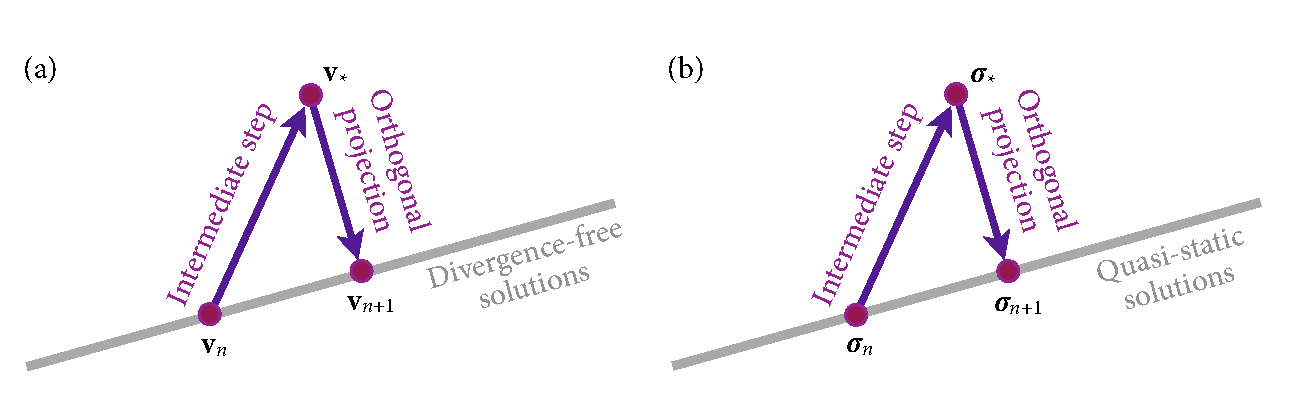
\includegraphics[width=\textwidth]{proj_diagram}
  \caption{Schematic of the timestep in (a) the projection method for
  incompressible fluid mechanics and (b) quasi-static
  elastoplasticity.\label{fig:ortho}}
\end{figure}

\section*{An inner product for the projection}
A key mathematical idea behind the fluid projection method is that for a
suitably chosen inner product, the projection that is applied is orthogonal to
the space of divergence-free solutions, as shown schematically in
Fig.~\ref{fig:ortho}(a). This ensures that during the numerical scheme, the
projection does apply any additional changes to the velocity field. The inner
product that is used for this purpose is
\begin{equation}
  \langle \vec{a},\vec{b} \rangle = \int \vec{a} \cdot \vec{b} \, d^2 \vec{x}. \label{eq:fl_inner}
\end{equation}
In the method, the projection is proportional to $\nabla p$. By applying the
divergence theorem and neglecting any boundary contributions,
\begin{equation}
  \langle \vec{v}_{n+1} - \vec{v}_n, \nabla p \rangle =  \int (\vec{v}_{n+1} - \vec{v}_n) \cdot \nabla p \, d^2\vec{x}
  = \int ( \nabla \cdot \vec{v}_{n+1} - \nabla \cdot \vec{v}_{n} ) \cdot p \, d^2 \vec{x} = 0,\\
\end{equation}
and thus the projection is orthogonal to the diveregence-free solutions as
expected.

Figure~\ref{fig:ortho}(b) shows the corresponding schematic for quasi-static
elastoplasticity, whereby the projection should be orthogonal to the space of
quasi-static solutions. An appropriate inner product on the space of stress
fields is
\begin{equation}
  \langle \vec{a},\vec{b} \rangle = \int \left((3\lambda + 2 \mu) \vec{a} : \vec{b} - \lambda(\tr \vec{a}) \cdot (\tr \vec{b}) \right) d^2\vec{x}
  \label{eq:qs_inner}
\end{equation}
where \smash{$\lambda=K-\frac{2}{3}\mu$} is Lam\'e's first parameter. Even
though the second term in the integrand is negative, the inner product is
positive definite as long as $\lambda$ and $\mu$ are positive, since the first
term dominates. Proving that Eq.~\ref{eq:qs_inner} is a suitable inner product
can be done following similar steps as for Eq.~\ref{eq:fl_inner}, by using
the divergence theorem to move derivatives from the projection over to the
stresses.

\section*{Measuring the size of the projection}
The inner product defined in Eq.~\ref{eq:qs_inner} provides a way to measure
the size of the projection, which may be useful in determining to what degree
the system is behaving quasi-statically. Suppose that in timestep $\Delta t$,
the projection that is applied is $\Dsig$. Furthermore, to properly handle
boundary terms, consider that the inner product is taken over a domain $S$. Then an appropriate measure of
quasi-staticity is
\begin{equation}
  Q = \frac{\sqrt{\langle \Dsig, \Dsig\rangle}}{\Delta T}
\end{equation}
and hence
\[
Q^2 = \frac{1}{\Delta T^2} \int_S \left( (3\lambda+2\mu) \Dsig: \Dsig - \lambda (\tr \Dsig)^2 \right) d^2\vec{x}.
\]
In terms of the components of $\Dsig$, this can be written as
\begin{eqnarray}
  Q^2 &=& \frac{1}{\Delta T^2} \int_S \left((3\lambda+2\mu) (3\pdel^2 +2 \sdel^2 + 2\taudel^2 + 6\qdel^2) - 9\lambda \pdel^2 \right) d^2\vec{x} \nonumber \\
  &=& \frac{1}{\Delta T^2} \int_S \left( (3\lambda+2\mu) (2 \sdel^2 + 2\taudel^2 + 6\qdel^2) + 6\mu \pdel^2 \right) d^2\vec{x} \nonumber \\
  &=& \frac{6}{\Delta T^2} \int_S \left( K(\sdel^2+\taudel^2 +3\qdel^2) + \mu \pdel^2 \right) d^2\vec{x} \nonumber \\
  &=& \frac{6}{\Delta T^2} \int_S \left( K\bar{s}_P^2 + \mu \pdel^2 \right) d^2 \vec{x}
\end{eqnarray}
By making use of Eqs.~\ref{eq:proj_start} to \ref{eq:proj_end}, this can be
written in terms of velocities as
\begin{eqnarray}
  Q^2 &=& 6 \int_S \left( K\mu^2 \left( (U_x-V_y)^2 + (U_y+V_x)^2 + \tfrac{1}{3} (U_x+V_y)^2 \right) + K^2\mu (U_x+V_y)^2 \right) d^2\vec{x} \\
  &=& 6K\mu \int_S \left( K'(U_x+V_y)^2 + \mu \left((U_x-V_y)^2 + (U_y+V_x)^2 \right) \right) d^2\vec{x} \\
  &=& 6K\mu \int_S \left( \mu (U_x^2 + U_y^2+ V_x^2 + V_y^2 - 2U_xV_y+2U_yV_x) + K'(U_x^2 + 2U_x V_y + V_y^2) \right) d^2 \vec{x}, \label{eq:projvel}
\end{eqnarray}
where \smash{$K'=K+\frac{\mu}{3}$} as defined above. Equation~\ref{eq:projvel}
may be a useful form to evaluate $Q$. The derivatives of velocity are already
calculated within the code and the spatial distribution of the integrand could
be examined. An alternative form can also be derived in terms of stresses by
first considering the expression
\begin{eqnarray}
\frac{\Dsig \vec{U}}{\Delta T} &=& \left(
\begin{array}{ccc}
  K'(U_x+V_y) + \mu(U_x - V_y) & \mu (U_y+V_x) & 0 \\
  \mu(U_y+V_x) & K'(U_x + V_y) - \mu(U_x - V_y) & 0 \\
  0 & 0 & \lambda (U_x+V_y)
\end{array}
\right)
\left(
\begin{array}{c}
  U \\ V \\ 0
\end{array}
\right) \nonumber \\
&=& \left(
\begin{array}{c}
  K'U(U_x+V_y) + \mu U (U_x-V_y) + \mu V(U_y+V_x) \\
  \mu U (U_y+V_x) + K'V (U_x+V_y) - \mu V (U_x - V_y) \\
  0
\end{array}
\right). \label{eq:divexp}
\end{eqnarray}
Taking the divergence of Eq.~\ref{eq:divexp} will yield many of the same terms
as are present in Eq.~\ref{eq:projvel}. Hence, by using the divergence theorem,
\begin{eqnarray*}
  \frac{1}{\Delta T} \int_{\p S} \vec{U} \cdot \Dsig \cdot \vnor \, ds &=& \frac{1}{\Delta T} \int_S \nabla \cdot (\Dsig \vec{U}) d^2\vec{x} \\
   &=& \frac{Q^2}{6K\mu} +  \int_S \Big( U ( (\mu+K') U_{xx} + \mu U_{yy} + K'V_{xy}) \\
   &&+ V(\mu V_{xx} + (\mu+K') V_{yy} + K' U_{xy}) \Big) d^2 \vec{x} \\
   &=& \frac{Q^2}{6K\mu} + \frac{1}{\Delta T} \int_S \vec{U} \cdot (\nabla \cdot \bsig_*) \, d^2 \vec{x},
\end{eqnarray*}
where on the final line Eqs.~\ref{eq:double_multi1} and \ref{eq:double_multi2}
have been substituted. Hence $Q$ can be written in terms of stresses and
velocities as
\begin{equation}
  \frac{Q^2 \, \Delta T}{6K\mu} = \int_{\p S} \vec{U} \cdot \Dsig \cdot \vnor \,ds - \int_S \vec{U} \cdot (\nabla \cdot \bsig_*) \, d^2 \vec{x}.
\end{equation}
Note that this expression involves both the intermediate stress $\bsig_*$ and
the stress projection $\Dsig$.

\bibliography{bmg}

\end{document}
